
\documentclass[11pt]{article}

\usepackage[margin=1in]{geometry}
\usepackage{authblk}
\usepackage{booktabs}
\usepackage{graphicx}
\usepackage{lineno}
\usepackage{natbib}
\usepackage{amsmath}
\usepackage{amssymb}
\usepackage{siunitx}
\usepackage{xcolor}
\usepackage{longtable}

\linenumbers

\title{On the Forecasting of Record-Breaking Extremes: Benchmarking Probabilistic AI Weather Forecasts}
\author[1]{Author list to be finalized}
\affil[1]{Affiliations to be finalized}
\date{}

\begin{document}
\maketitle

\begin{abstract}

AI-based ensemble weather prediction systems now rival traditional numerical weather prediction on many medium-range benchmarks, but their reliability for unprecedented extremes remains unclear. We extend the deterministic record-extreme framework of \citet{zhang2026recordextremes} to probabilistic ensemble forecasts of record-breaking heat, cold, and wind. Using 2022 forecasts at 1.5$^{\circ}$ resolution, with monthly local records defined from ERA5 over 1979--2018, we evaluate the physics-based ensemble IFS-ENS and three AI ensembles, FGN, U-Cast, and ArchesWeatherGen. The analysis combines point-summary errors, record-occurrence probabilities, Brier scores, reliability summaries, precision-recall diagnostics, continuous ranked probability scores, and margin-conditioned tail diagnostics, including out-of-ensemble rates and ensemble coverage. Record-breaking events emerge as a distinct verification regime from average weather, and forecast performance depends strongly on event type, lead time, season, and land-sea class. Some AI ensembles represent heat-record occurrence and intensity competitively, but cold records and especially wind records remain more fragile, particularly for large record margins. These results show that probabilistic AI weather forecasts should be assessed not only by whether they predict record exceedance, but also by whether their predictive distributions credibly reach the observed record intensity.
\end{abstract}

\section{Introduction}

Reliable forecasts of record-breaking extremes are essential for early warning, public health, energy systems, agriculture, transport and disaster response. Their importance has been underscored by the ongoing 2026 heat extremes: Copernicus reported that western Europe experienced its hottest June on record during an intense regional heatwave, while the month ranked as the second warmest globally. At the same time, WMO documented concurrent heat impacts, wildfire risk and record temperatures across multiple countries \citep{c3s2026juneheat,wmo2026europeheat}. Against this backdrop, a central forecasting question is whether modern forecast systems remain credible when the atmosphere produces conditions beyond the local seasonal range represented in historical data.

Recent AI weather prediction systems have transformed traditional forecasting systems. Deterministic models such as GraphCast, Pangu-Weather, and FuXi achieved strong global skill at a fraction of the computational cost of traditional numerical weather prediction in many benchmark settings \citep{rasp2024weatherbench2,lam2023graphcast, bi2023pangu, chen2023fuxi}. Yet strong average skill does not imply strong tail skill. A model can reduce global error by forecasting ordinary weather well while still failing in the rare, high-impact situations for which warning performance matters most.

Very recently, that failure mode was made explicit by \citet{zhang2026recordextremes}. They defined record-breaking heat, cold, and wind events locally relative to each grid cell and calendar month, then asked whether deterministic forecasts could predict values beyond the previous historical record. Their conclusion was clear: the physics-based ECMWF deterministic forecast HRES outperformed GraphCast, Pangu-Weather, and FuXi for record-breaking events across heat, cold, and wind. The AI forecasts tended to underpredict hot records, overpredict cold records, and underpredict wind records, with the errors worsening as the observed margin beyond the previous record increased. This pattern suggests a ``soft cap'' in which models trained on historical reanalysis remain excellent interpolators but struggle to extrapolate beyond the training range.

A next question to be addressed by the research community is therefore probabilistic. Weather is chaotic, and high-impact decisions require probabilistic rather than point forecasts. Probabilistic AI systems such as GenCast, FGN, U-Cast, ArchesWeatherGen, FuXi-ENS, and AIFS-CRPS produce ensembles or predictive distributions and are often trained with objectives related to proper scoring rules \citep{price2025gencast, alet2026operational, ruhlingcachay2026ucast, couairon2026arches, zhong2025fuxiens, lang2026aifscrps}. In principle, such systems may place probability mass beyond the historical record even when their ensemble mean remains conservative. In practice, they may still be underdispersive, miscalibrated in the tails, or unable to place support near the observed intensity of unprecedented events. That distinction matters scientifically and operationally: assigning nonzero probability to record exceedance is not the same as providing a calibrated forecast distribution for the resulting event severity.

This study extends the deterministic record-extreme benchmark to probabilistic ensemble forecasts. We evaluate the physics-based ensemble IFS-ENS together with three AI ensembles, FGN, U-Cast, and ArchesWeatherGen, using evluation metrics: point forecast summaries, record-occurrence metrics, CRPS, and margin-conditioned tail diagnostics. 

\section{Data and methods}

In the present study, monthly records are computed from ERA5 over the reference period 1979--2018. The main variables of interest are 2m temperature and 10m wind speed. Heat records are upper records of 2m temperature, cold records are lower records of 2m temperature, and wind records are upper records of 10m wind speed. The spatial domain is restricted to the no-Antarctic 1.5$^{\circ}$ grid, approximately $60^{\circ}$S to $90^{\circ}$N. The temporal domain is restricted to 00 and 12 UTC valid times, and we use 2022 as test set.

More formally, let $x_{s,t}$ denote a weather variable at grid cell $s$ and verification time $t$. For variable $x$, grid cell $s$, and calendar month $m$, define the historical upper record over the reference period $T_{\mathrm{train}}$ (1979--2018) as
\begin{equation}
    r^{x,+}_{s,m} = \max_{t \in T_{\mathrm{train}}: m(t)=m} x_{s,t},
    \label{eq:upperrecord}
\end{equation}
and the lower record as
\begin{equation}
    r^{x,-}_{s,m} = \min_{t \in T_{\mathrm{train}}: m(t)=m} x_{s,t}.
    \label{eq:lowerrecord}
\end{equation}
An upper-tail record in the test year occurs at $(s,t)$ if
\begin{equation}
    y^{+}_{s,t} = \mathbb{1}\{x_{s,t} > r^{x,+}_{s,m(t)}\}=1,
    \label{eq:upperindicator}
\end{equation}
whereas a lower-tail record occurs if
\begin{equation}
    y^{-}_{s,t} = \mathbb{1}\{x_{s,t} < r^{x,-}_{s,m(t)}\}=1.
    \label{eq:lowerindicator}
\end{equation}
The test set is therefore composed of grid-time pairs that are unprecedented relative to the local seasonal historical range of 1979--2018. 

The processed forecast set contains the ECMWF's physics-based IFS-ENS ensemble and three probabilistic AI systems: FGN, ArchesWeatherGen, and U-Cast~\citep{alet2026operational,couairon2026arches,ruhlingcachay2026ucast}. At a high level, the three models represent three major directions in AI-based weather forecasting: FGN uses a graph-transformer architecture, with a graph neural network mapping latitude-longitude fields to a multilevel icosahedral mesh and a graph-transformer processor operating there; its probabilistic character comes from learned, globally shared functional perturbations of the network parameters, combined with a deep ensemble, allowing it to model forecast uncertainty while optimizing the continuous ranked probability score (CRPS). ArchesWeatherGen uses a 3D Swin U-Net transformer on the atmospheric latitude-longitude-vertical grid, enhanced with cross-level attention, and generates ensembles through flow matching: a deterministic ArchesWeather prediction provides the mean state while a generative model samples the residual uncertainty and is rolled out autoregressively. U-Cast, on the other hand, uses a conventional convolutional U-Net with bottleneck self-attention, Monte Carlo dropout for stochasticity, and a deterministic-to-probabilistic training curriculum from mean absolute error (MAE) to CRPS. 

\subsection{Evaluation and metrics}

IFS-ENS is evaluated with 50 members. FGN, U-Cast, and ArchesWeatherGen are evaluated with 64 members. The processed lead times are 12, 48, 120, 168, and 240 h for IFS-ENS, FGN, and U-Cast, with 12-hourly data missing for ArchesWeatherGen. Moreover, IFS-ENS is verified against HRES-fc0, the deterministic ECMWF forecast initialized at the same time as the ensemble. FGN, U-Cast, and ArchesWeatherGen are verified against ERA5. Below we discuss the different evaluation metrics used to assess the (probabilistic) forecasts. 

\subsubsection{Point forecasts}

An ensemble forecast with $K$ members for variable $x$ at grid cell $s$, initialization time $t_0$, and lead time $\tau$ is
\begin{equation}
    \left\{\hat{x}^{\tau,1}_{s,t_0}, \ldots, \hat{x}^{\tau,K}_{s,t_0}\right\}.
\end{equation}
It can be collapsed to a point forecast using the ensemble mean,
\begin{equation}
    \bar{x}^{\tau}_{s,t_0} = \frac{1}{K}\sum_{k=1}^{K}\hat{x}^{\tau,k}_{s,t_0},
    \label{eq:ensmean}
\end{equation}
or the ensemble median. This reduction is useful for comparison with deterministic benchmarks, but it discards the predictive distribution and can be misleading because ensemble means are often smoother than individual members.

For an evaluation set $I$, the latitude-weighted RMSE of a point forecast $\tilde{x}^{\tau}_{s,t_0}$ is
\begin{equation}
    \mathrm{RMSE}_I(\tau) =
    \left\{
    \frac{\sum_{(s,t_0)\in I} \omega_s\left(\tilde{x}^{\tau}_{s,t_0} - x_{s,t_0+\tau}\right)^2}
    {\sum_{(s,t_0)\in I} \omega_s}
    \right\}^{1/2},
    \label{eq:rmse}
\end{equation}
where $\omega_s$ is the latitude weight. The corresponding bias is
\begin{equation}
    \mathrm{Bias}_I(\tau) =
    \frac{\sum_{(s,t_0)\in I} \omega_s\left(\tilde{x}^{\tau}_{s,t_0} - x_{s,t_0+\tau}\right)}
    {\sum_{(s,t_0)\in I} \omega_s}.
    \label{eq:bias}
\end{equation}
We evaluate these scores on all valid grid-time pairs and on the observed-record sets. 

\subsubsection{Occurence probabilities}

For upper-tail records, the ensemble probability of breaking the historical record is
\begin{equation}
    \hat{p}^{\tau,+}_{s,t_0} = \frac{1}{K}\sum_{k=1}^{K}
    \mathbb{1}\left\{\hat{x}^{\tau,k}_{s,t_0} > r^{x,+}_{s,m(t_0+\tau)}\right\}.
    \label{eq:probupper}
\end{equation}
For lower-tail records, the inequality is reversed. The occurrence problem is then a rare-event probabilistic classification problem: the forecast is $\hat{p}^{\tau}_{s,t_0}$ and the observation is $y^{\tau}_{s,t_0}\in\{0,1\}$.

For an evaluation set $I$, the weighted observed and expected record counts are
\begin{equation}
    N^{\tau}_I = \sum_{(s,t_0)\in I}\omega_s y^{\tau}_{s,t_0}, \qquad
    \hat{N}^{\tau}_I = \sum_{(s,t_0)\in I}\omega_s \hat{p}^{\tau}_{s,t_0}.
    \label{eq:counts}
\end{equation}
The difference $\hat{N}^{\tau}_I - N^{\tau}_I$ diagnoses whether records are over- or underforecast in expectation. 

\subsubsection{Precision, recall, and the forecaster's dilemma}

For a probability cutoff $c$, a record alarm is
\begin{equation}
    \hat{y}^{\tau}_{s,t_0}(c) = \mathbb{1}\left\{\hat{p}^{\tau}_{s,t_0} > c\right\}.
    \label{eq:alarm}
\end{equation}
Precision and recall are
\begin{equation}
    \mathrm{Precision}(c)=\frac{\mathrm{TP}(c)}{\mathrm{TP}(c)+\mathrm{FP}(c)}, \qquad
    \mathrm{Recall}(c)=\frac{\mathrm{TP}(c)}{\mathrm{TP}(c)+\mathrm{FN}(c)}.
    \label{eq:pr}
\end{equation}
Precision-recall curves are preferable to ROC curves for these rare events because true negatives dominate the global grid-time sample. In an early-warning setting, the high-precision, moderate-recall part of the curve is often especially relevant: a forecast that catches many records only by issuing alarms nearly everywhere is practically useless even if recall is high.

Because record-conditioned scoring selects on the observed outcome, it must be interpreted alongside full-sample occurrence diagnostics and forecast-conditioned checks. This is the practical implication of the forecaster's dilemma \citep{holzmann2014information,lerch2017forecasters}: evaluating only observed extremes can reward overforecasting. In this work, record-conditioned scores are therefore treated as stress tests rather than standalone decision rules.

\subsubsection{Brier score and reliability}

The Brier score evaluates the numerical record probability directly \citep{brier1950verification}:
\begin{equation}
    \mathrm{BS}_I(\tau)=
    \frac{\sum_{(s,t_0)\in I}\omega_s\left(\hat{p}^{\tau}_{s,t_0}-y^{\tau}_{s,t_0}\right)^2}
    {\sum_{(s,t_0)\in I}\omega_s}.
    \label{eq:brier}
\end{equation}
The Murphy decomposition separates the Brier score into uncertainty, reliability, and resolution components \citep{murphy1973partition}.

Reliability diagrams group predictions into probability bins and compare the mean predicted probability $\bar{p}_b$ with the observed event frequency $\bar{y}_b$. The current bins are deliberately small near zero:
\begin{align}
    &[0,0.001), [0.001,0.01), [0.01,0.02), [0.02,0.05), [0.05,0.10), \\
    &[0.10,0.20), [0.20,0.40), [0.40,0.60), [0.60,0.80), [0.80,1].
\end{align}
This resolution near zero is important because a probabilistic soft cap would appear most clearly when observed records receive zero or near-zero forecast probability.

\subsubsection{Zero-probability miss rate}

Reliability at $\hat{p}=0$ can look deceptively good because record events are rare. The more operationally relevant quantity for the soft-cap question is the reverse conditional probability
\begin{equation}
    \Pr(\hat{p}^{\tau}=0 \mid y^{\tau}=1),
    \label{eq:zeromiss}
\end{equation}
the fraction of observed records for which no ensemble member crossed the historical record. Equivalently,
\begin{equation}
    \Pr(\hat{p}^{\tau}=0 \mid y^{\tau}=1)=1-\mathrm{Recall}(c=0).
\end{equation}
This metric directly asks whether the event was inside the ensemble support at all. It is especially useful for distinguishing an ensemble that is miscalibrated but at least assigns nonzero tail probability from one that completely misses the observed record.

\subsubsection{Continuous ranked probability score}

The continuous ranked probability score is a proper scoring rule for real-valued probabilistic forecasts \citep{gneiting2007strictly, jordan2019scoringrules}. For predictive distribution $F^{\tau}_{s,t_0}$ and observation $x_{s,t_0+\tau}$,
\begin{equation}
    \mathrm{CRPS}\left(F^{\tau}_{s,t_0}, x_{s,t_0+\tau}\right)
    = \int_{-\infty}^{\infty}\left(F^{\tau}_{s,t_0}(z)-\mathbb{1}\{x_{s,t_0+\tau}\le z\}\right)^2\,dz.
    \label{eq:crpscdf}
\end{equation}
It can be interpreted as an integral of threshold-specific Brier scores \citep{hersbach2000crps}. For an empirical ensemble with $K$ members,
\begin{equation}
    \widehat{\mathrm{CRPS}}_{s,t_0}^{\tau}
    = \frac{1}{K}\sum_{k=1}^{K}\left|\hat{x}^{\tau,k}_{s,t_0}-x_{s,t_0+\tau}\right|
    - \frac{1}{2K^2}\sum_{k=1}^{K}\sum_{\ell=1}^{K}
    \left|\hat{x}^{\tau,k}_{s,t_0}-\hat{x}^{\tau,\ell}_{s,t_0}\right|.
    \label{eq:crpsempirical}
\end{equation}
The first term rewards ensemble members close to the verification, and the second term accounts for ensemble spread. In the deterministic limit, CRPS reduces to the mean absolute error. 

\subsubsection{Record margin and tail-coverage}

For upper-tail records, define the observed record margin as
\begin{equation}
    e^{+}_{s,t}=x_{s,t}-r^{x,+}_{s,m(t)}.
    \label{eq:marginupper}
\end{equation}
For lower-tail records,
\begin{equation}
    e^{-}_{s,t}=r^{x,-}_{s,m(t)}-x_{s,t}.
    \label{eq:marginlower}
\end{equation}
For a margin threshold $u$, diagnostics are computed over records with $e_{s,t}>u$. If an ensemble is subject to a probabilistic soft cap, bias and out-of-ensemble rates should worsen as $u$ increases.

In addition to CRPS, RMSE, and bias as functions of $u$, the margin outputs store the mean predicted record probability, the out-of-ensemble rate, and 90\% ensemble coverage. For an upper record, the out-of-ensemble indicator is
\begin{equation}
    \mathbb{1}\left\{x_{s,t_0+\tau} > \max_{1\le k\le K}\hat{x}^{\tau,k}_{s,t_0}\right\},
\end{equation}
with the inequality reversed for lower records. The 90\% coverage diagnostic checks whether the verifying value falls between the empirical 5th and 95th percentiles of the ensemble. Together these diagnostics show whether the observed record is not merely above the threshold but represented at the observed intensity within the predictive distribution.

\section{Results}

\subsection{Point Summaries Recover Lead-Dependent Record Attenuation}

We first collapse each ensemble to its mean, following the point-forecast perspective of \citet{zhang2026recordextremes}. This is a useful bridge to deterministic verification, but it deliberately discards ensemble spread and probability information. Across all-domain, all-season record events, RMSE increases with lead time and the signed biases have the expected attenuating direction: heat and wind records are too cold and too weak, whereas cold records are too warm (Figure~\ref{fig:pointskill}). The result is shared by the physics-based and AI ensembles, although its magnitude differs by event type and lead time. Thus, probabilistic sampling alone does not remove the point-forecast record-extreme problem.

The complete seasonal and land--sea inventory shows substantial heterogeneity. In particular, JJA land heat and DJF land cold records amplify the corresponding long-lead biases (Supplementary Figures~S1--S2). We use these point summaries as context for the probabilistic analysis below rather than as the primary test of an ensemble forecast.

\begin{figure}[t]
\centering
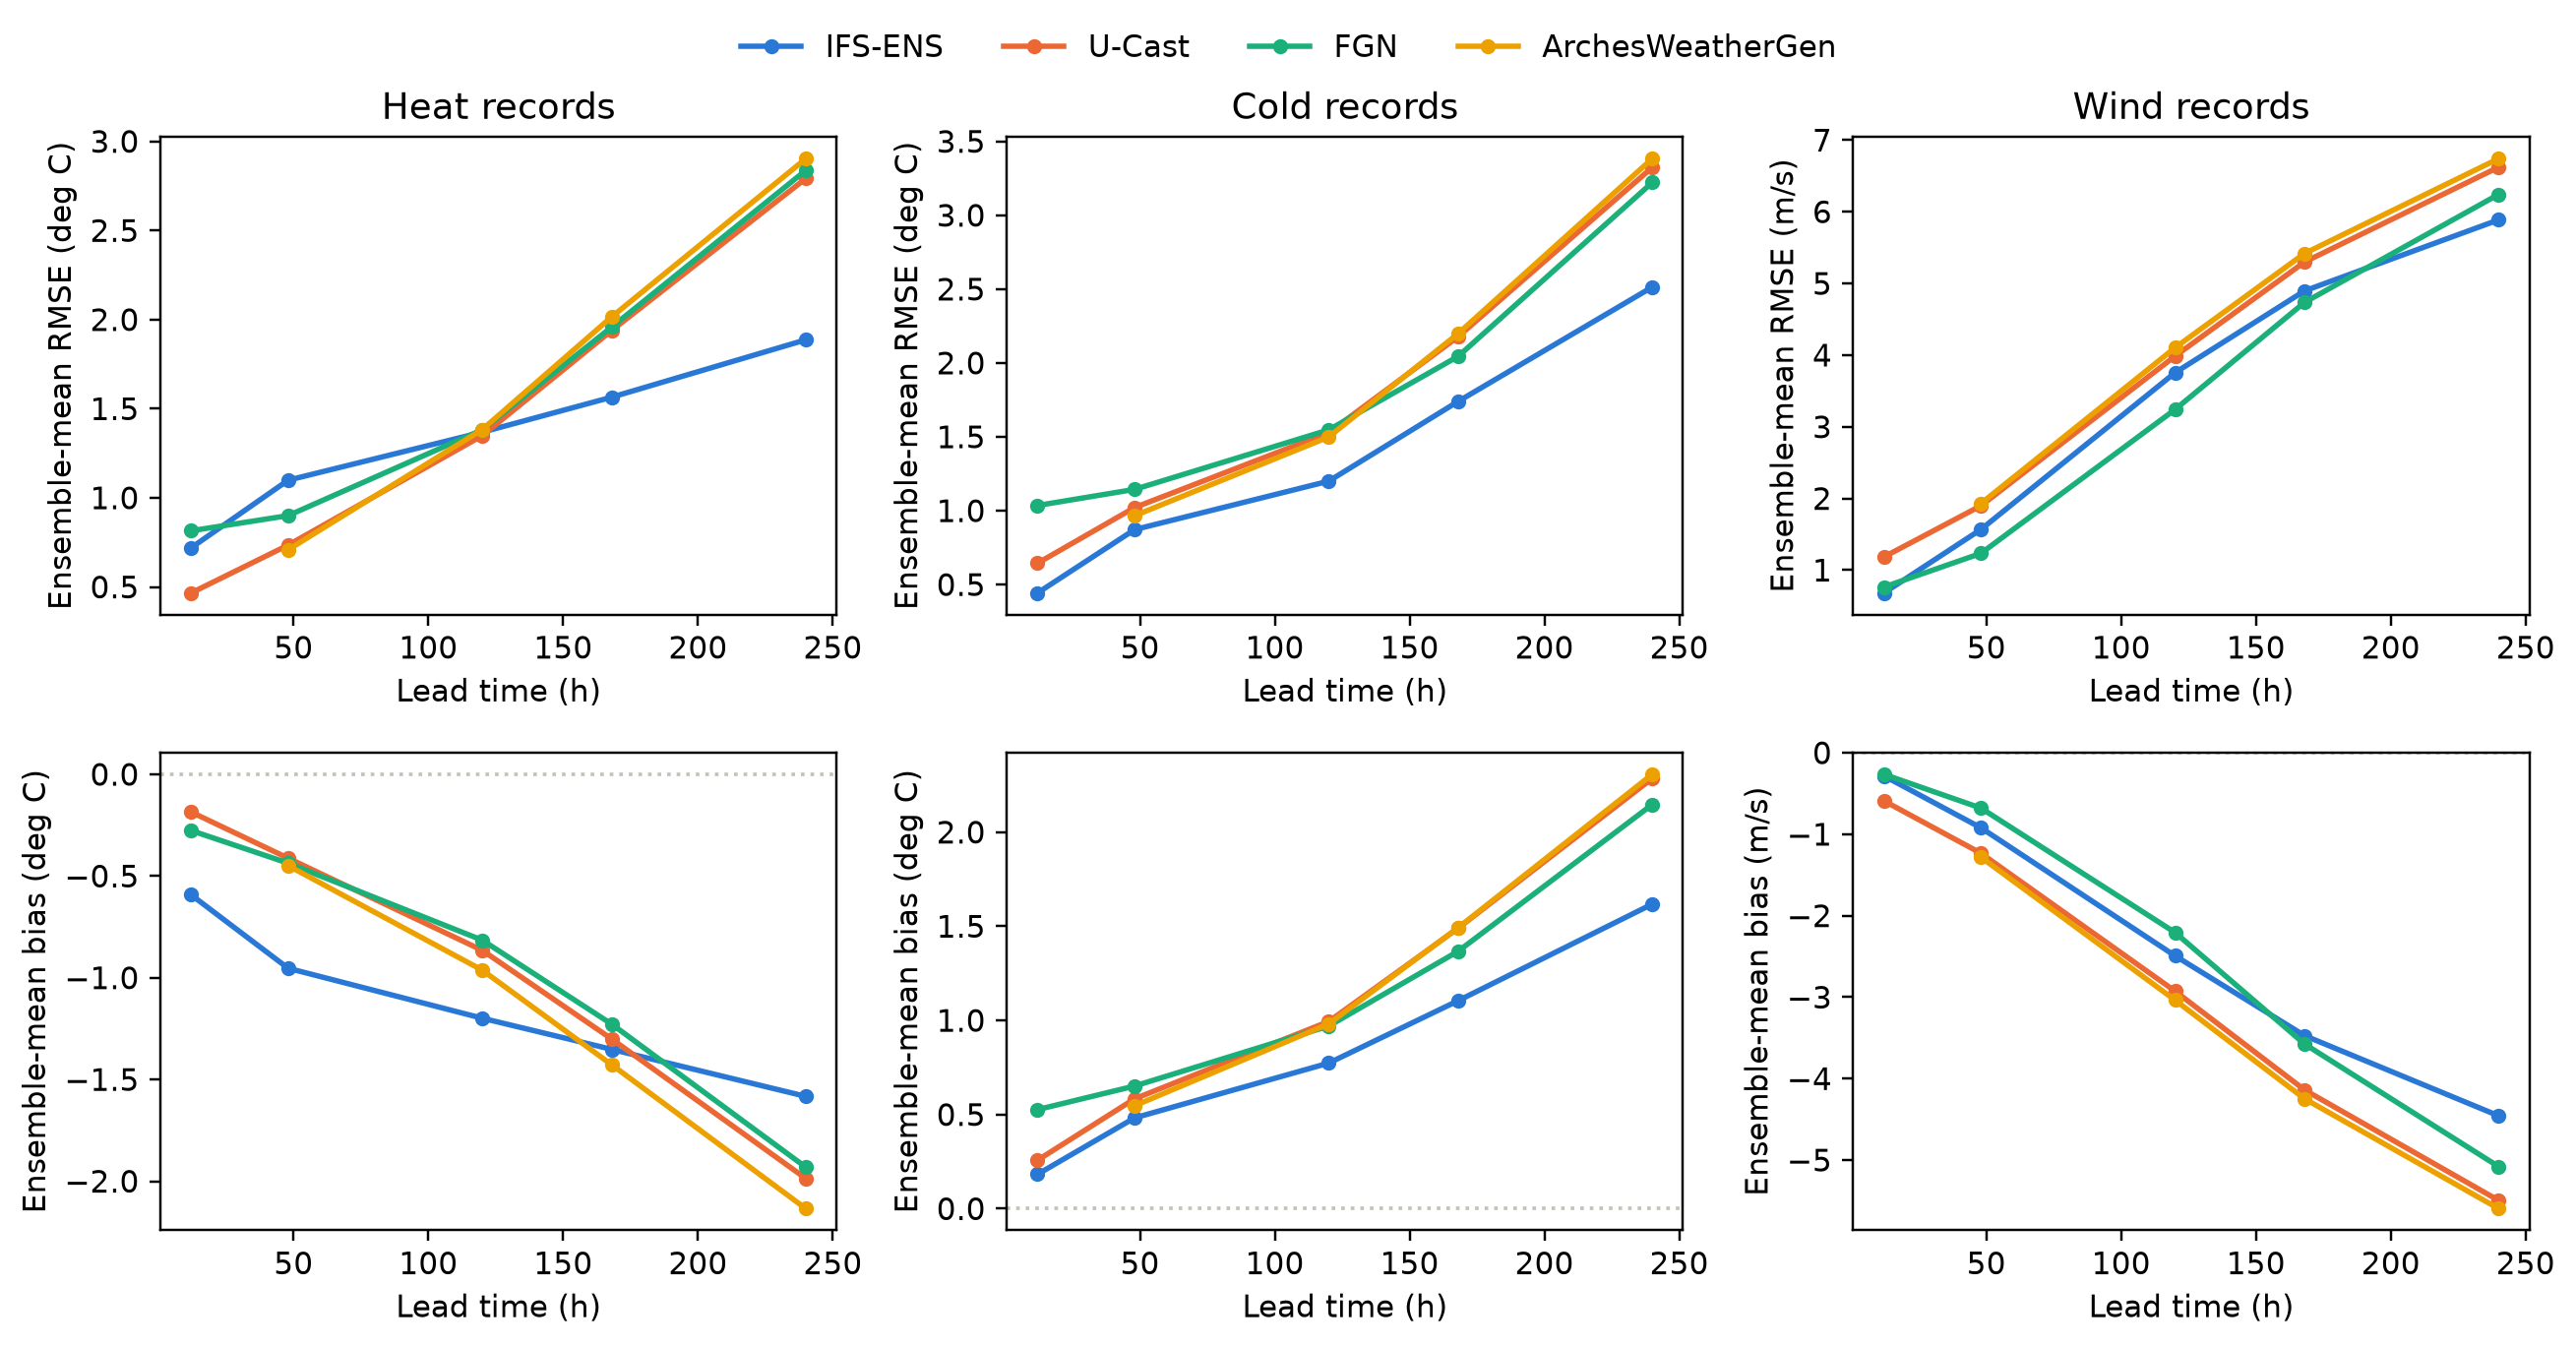
\includegraphics[width=0.96\linewidth]{fig/point_all_all.png}
\caption{All-domain, all-season ensemble-mean point skill for 2022 record events. Rows show RMSE and bias; columns show heat, cold, and wind records. Negative heat and wind bias and positive cold bias correspond to attenuation of record intensity.}
\label{fig:pointskill}
\end{figure}

\subsection{AI Ensembles Improve Record-Occurrence Forecasting, With Calibration Caveats}

The full ensemble changes the question from the predicted record value to the probability that a record occurs. Expected-minus-observed counts show that this probability mass is event- and lead-dependent (Figure~\ref{fig:counts}); the Brier score provides the more direct aggregate assessment of numerical probability quality (Figure~\ref{fig:brier}). Across the evaluated settings, the AI ensembles generally have lower Brier scores than IFS-ENS, most clearly for heat records. This is evidence that probabilistic AI can improve the anticipation of record occurrence, although the mixed verification targets require this comparison to be interpreted as a comparison of the current operational evaluation settings rather than a target-harmonized leaderboard.

At the common 48 h lead, precision--recall curves show that this difference is operationally relevant under the severe rarity of records, while reliability diagrams show that discrimination does not imply perfect calibration (Figure~\ref{fig:occurrence}). The AI systems can assign useful probability to heat and cold records, but some probability ranges, especially for wind, remain overconfident. Taken together, the occurrence diagnostics support an AI advantage for threshold anticipation, not a universal claim that every AI system is best in every regime.

\begin{figure}[t]
\centering
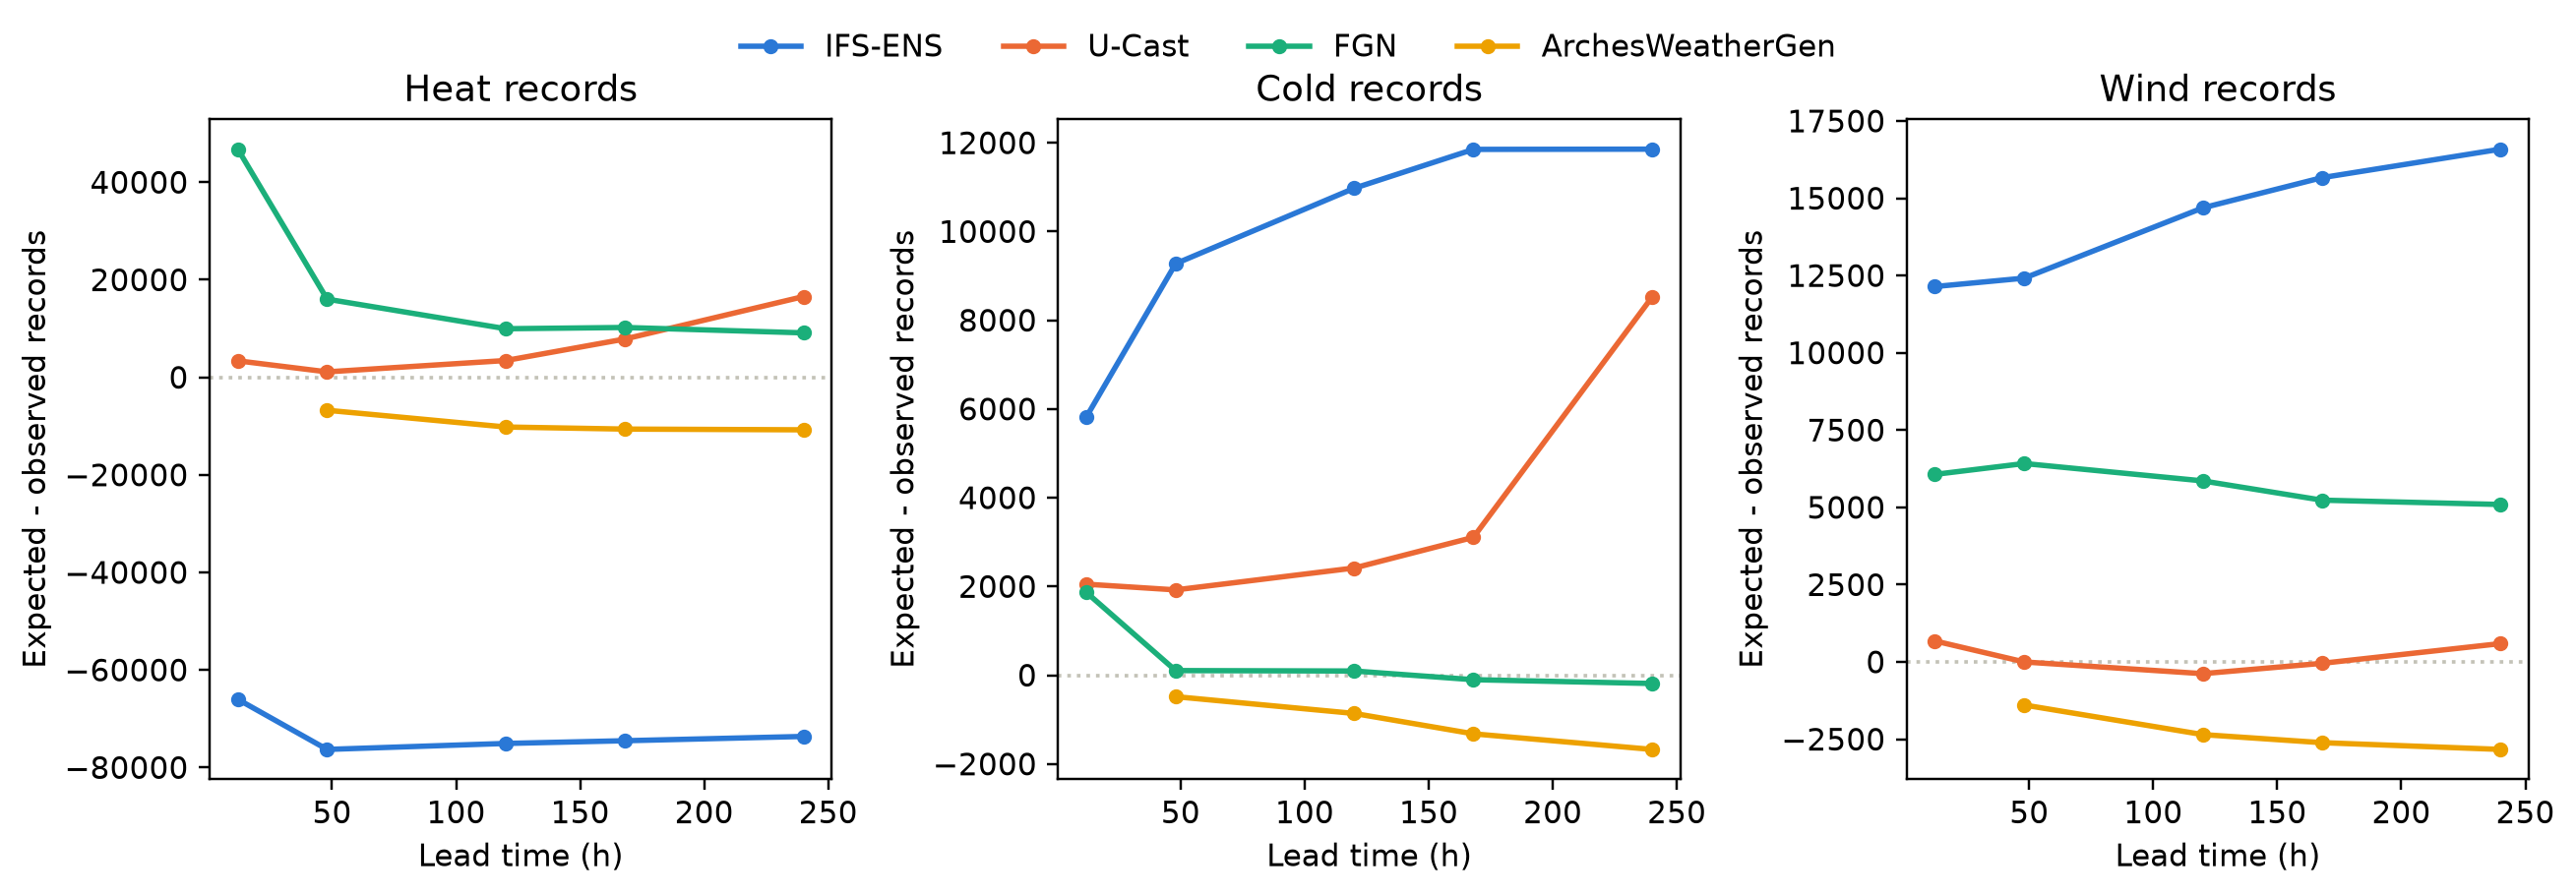
\includegraphics[width=0.96\linewidth]{fig/counts_all_all.png}
\caption{All-domain, all-season expected-minus-observed record counts. Positive values indicate that the ensemble assigns too much record probability in aggregate; negative values indicate too little.}
\label{fig:counts}
\end{figure}

\begin{figure}[t]
\centering
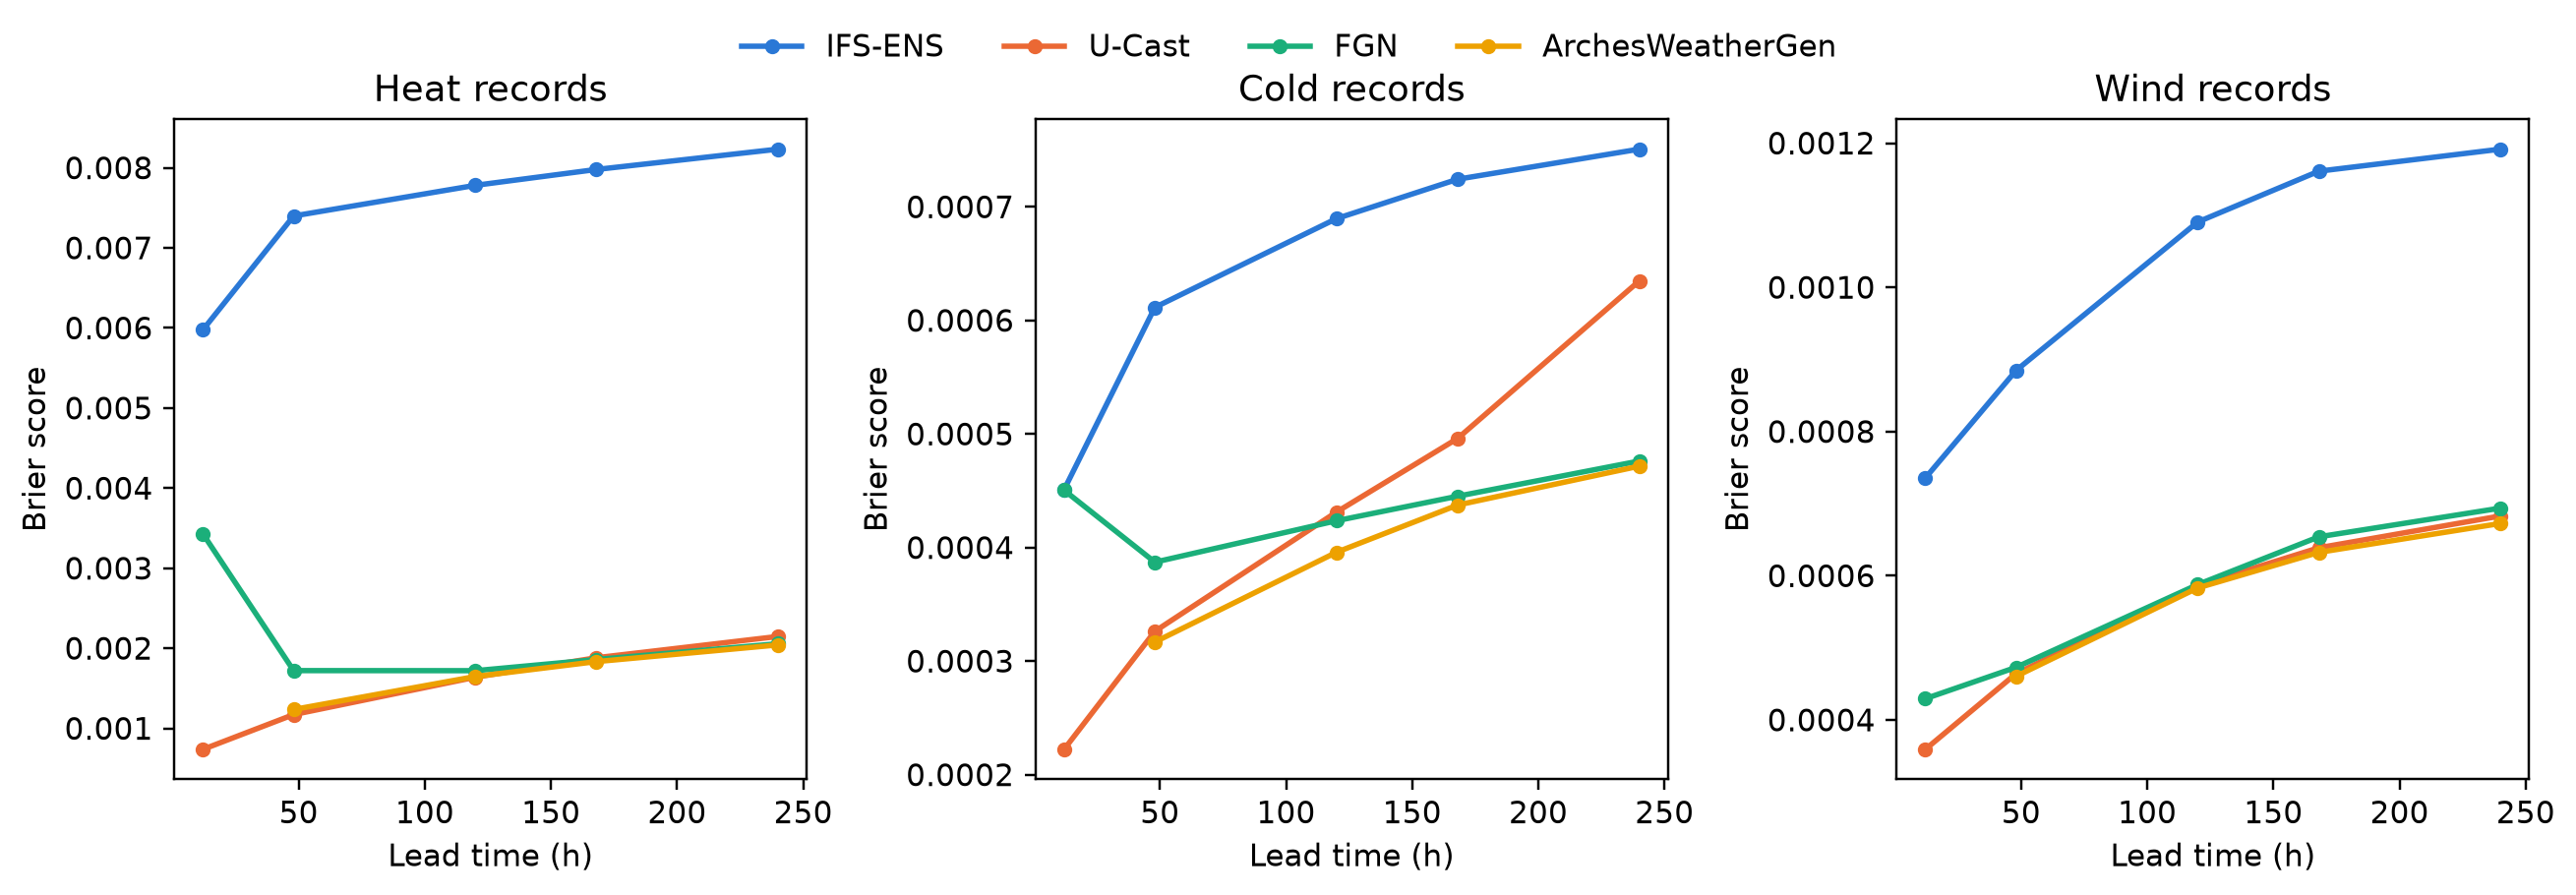
\includegraphics[width=0.96\linewidth]{fig/brier_all_all.png}
\caption{All-domain, all-season Brier scores for record occurrence. Lower values indicate more accurate numerical record probabilities.}
\label{fig:brier}
\end{figure}

\begin{figure}[t]
\centering
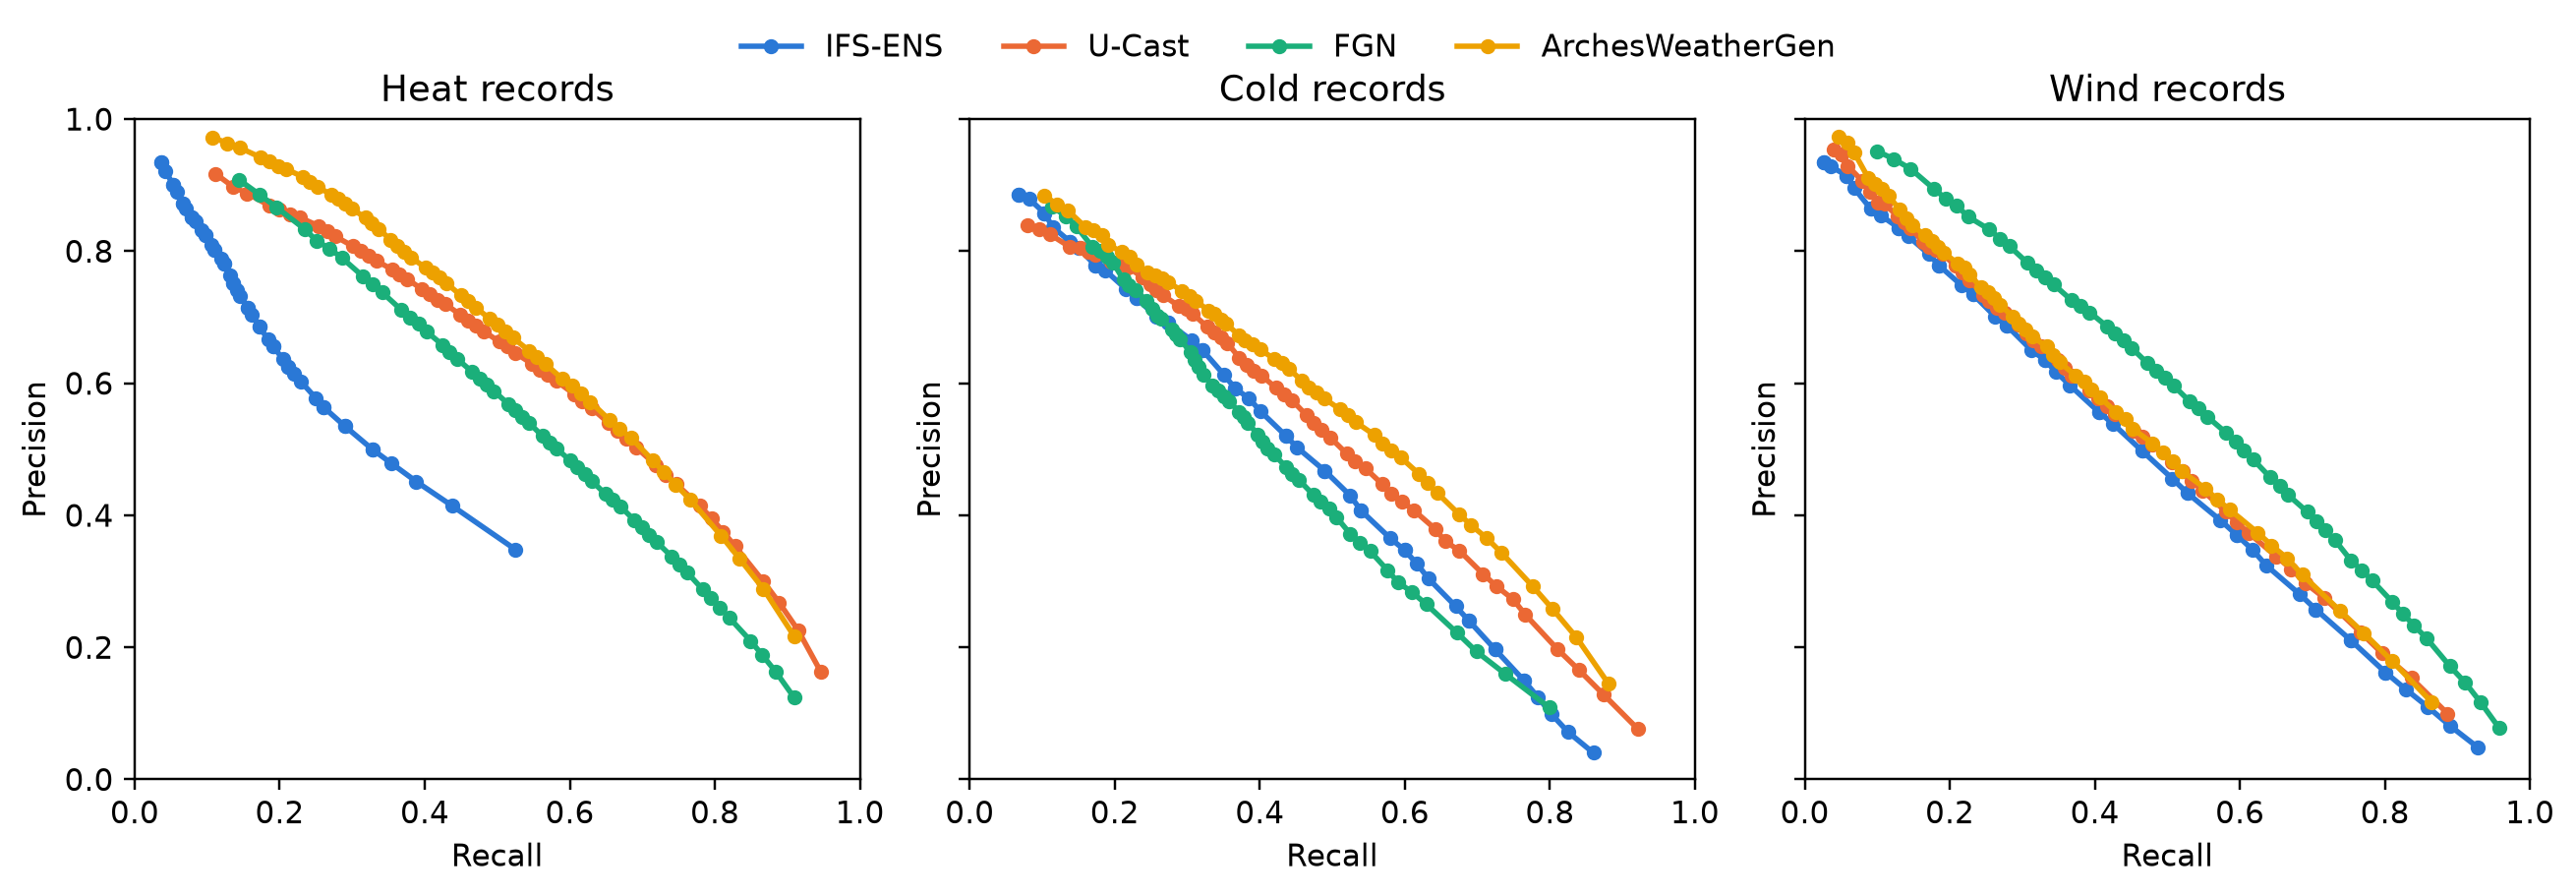
\includegraphics[width=0.96\linewidth]{fig/precision_recall_48h_all_all.png}
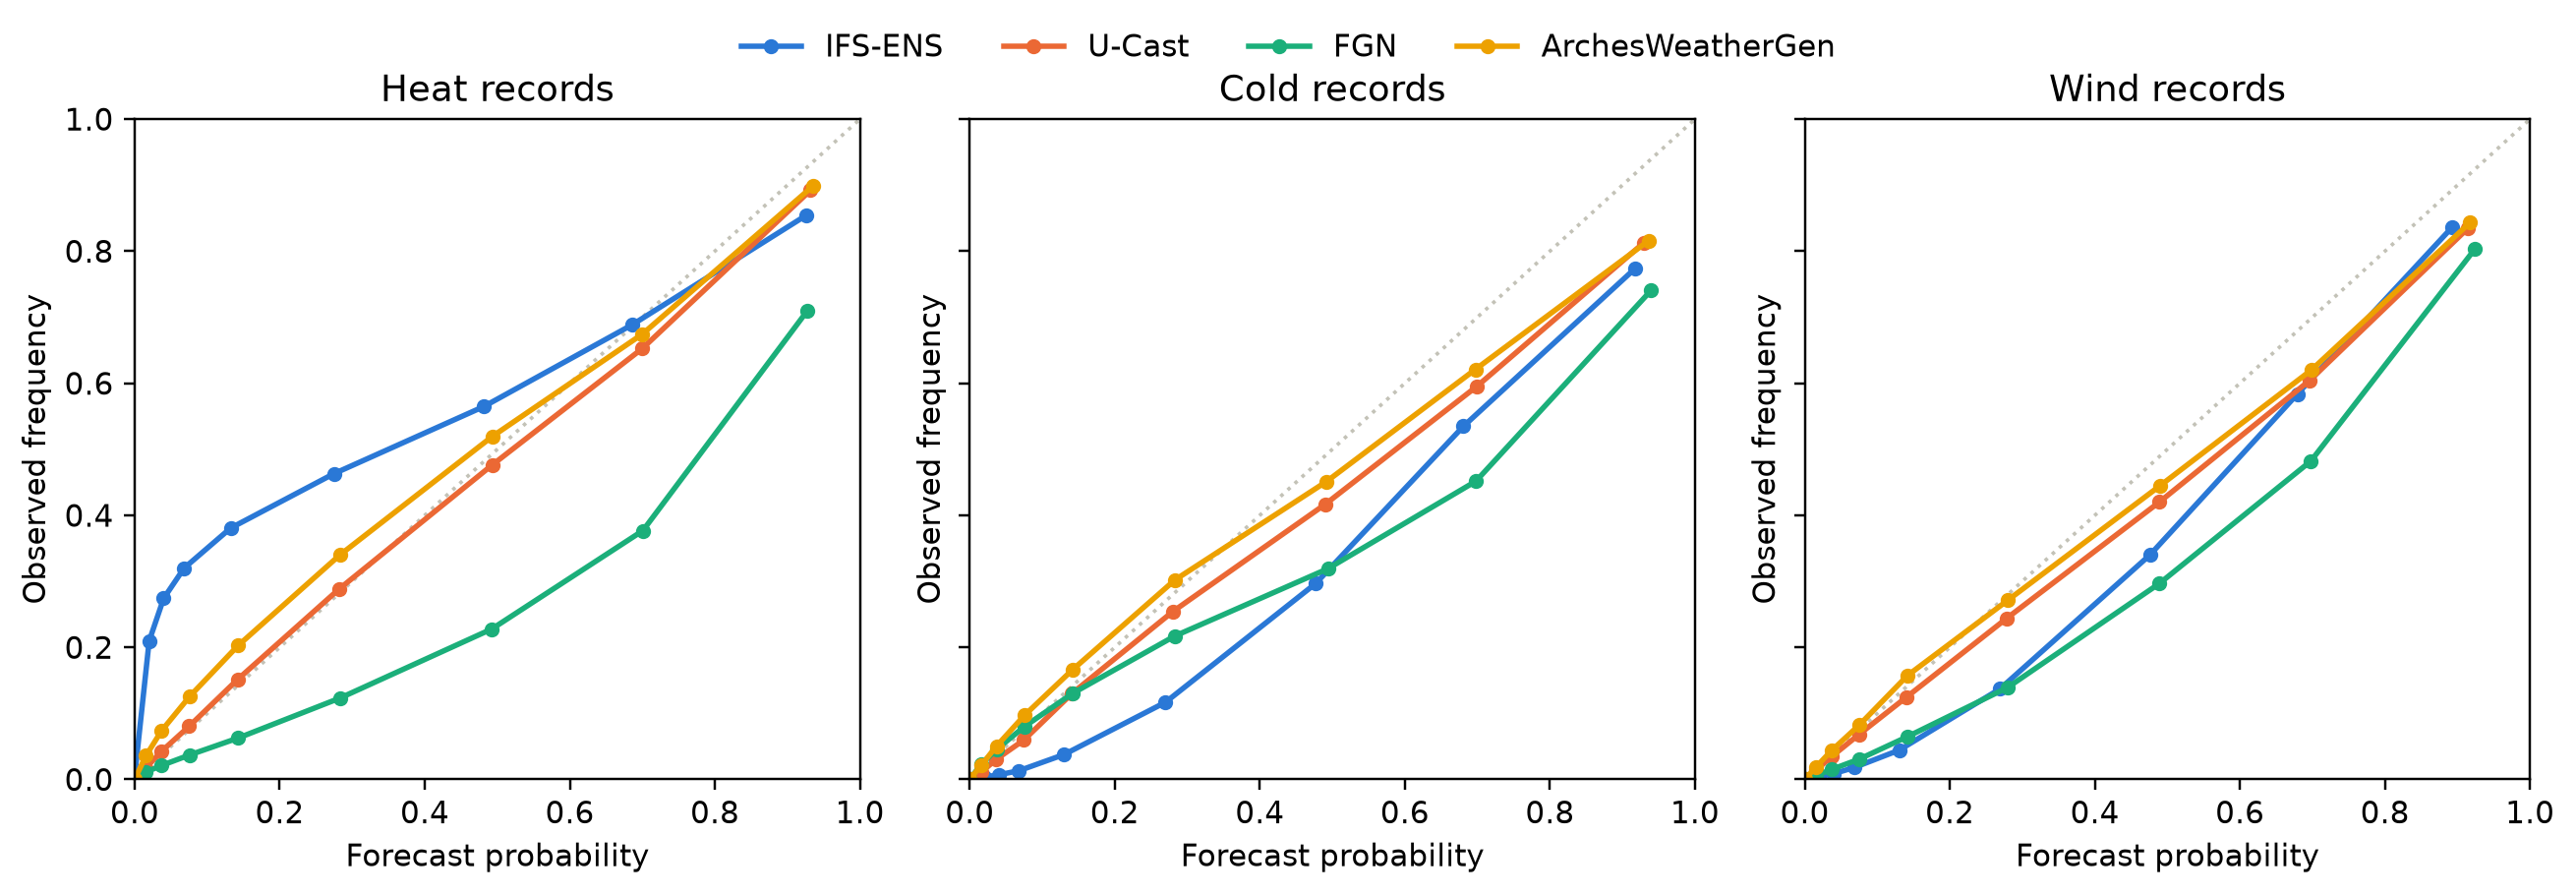
\includegraphics[width=0.96\linewidth]{fig/reliability_48h_all_all.png}
\caption{All-domain, all-season occurrence discrimination and calibration at 48 h. Top: precision--recall curves for probability-threshold alarms. Bottom: reliability diagrams; the diagonal denotes perfect calibration.}
\label{fig:occurrence}
\end{figure}

\subsection{Record-Conditioned Distributional Skill Remains Difficult}

CRPS assesses the full predictive distribution rather than its mean or its threshold-crossing probability. Record-conditioned CRPS (solid) is substantially larger than all-weather CRPS (dashed) for every event type and system, especially for wind at long lead (Figure~\ref{fig:crps}). Record extremes are therefore a distinct and harder probabilistic verification regime.

The occurrence advantage of AI does not translate uniformly into conditional intensity skill. At long leads, IFS-ENS remains competitive, and often stronger, for cold and wind record CRPS. Physics-based ensembles therefore remain appropriate when the operational question concerns the realized intensity conditional on a record occurring, rather than threshold occurrence alone.

\begin{figure}[t]
\centering
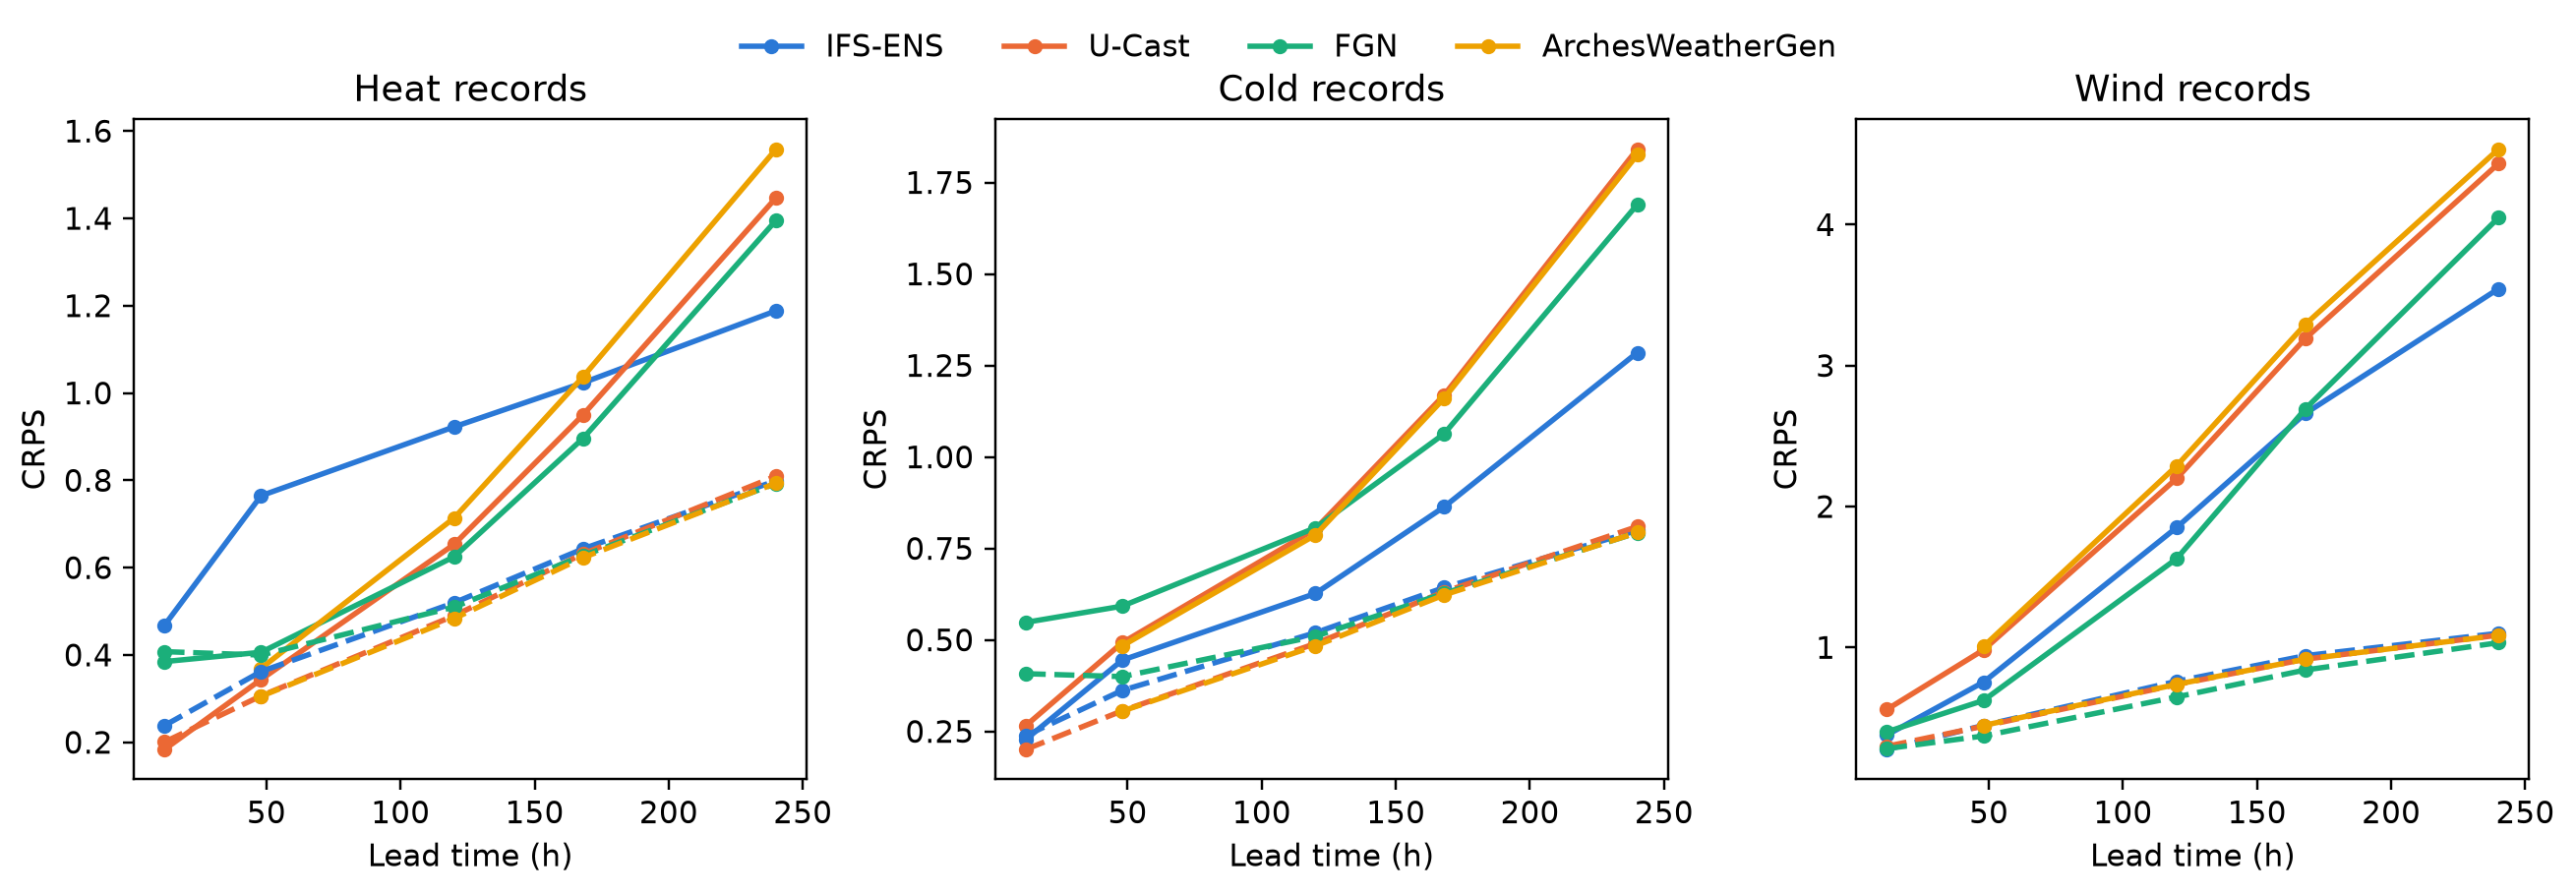
\includegraphics[width=0.96\linewidth]{fig/crps_all_all.png}
\caption{All-domain, all-season CRPS. Solid curves are conditioned on observed heat, cold, or wind records; dashed curves are all-weather CRPS. Lower values are better.}
\label{fig:crps}
\end{figure}

\subsection{Threshold Support Does Not Guarantee Intensity Support}

Margin-conditioned diagnostics provide the sharpest test of the probabilistic record-extreme hypothesis. As the observed record margin increases, CRPS and ensemble-mean error generally worsen in the attenuating direction (Figure~\ref{fig:margin-intensity}). Simultaneously, an ensemble can retain appreciable mean record probability while its coverage declines and its out-of-ensemble rate rises (Figure~\ref{fig:margin-probabilistic}).

For heat records at 120 h and a 4 K margin, the AI ensembles still assign mean record probabilities of roughly 0.77--0.85, but their empirical 90\% coverage is only about 0.13--0.30. Hence, an ensemble can anticipate that the historical threshold will be crossed while failing to extend sufficiently far into the realized tail. Cold and some wind margin subsets become sparse at large margins; those curves are retained as stress-test evidence in the Supplementary Materials rather than used for precise ranking.

The combined evidence gives a practical answer to the central question. Probabilistic AI improves record-occurrence forecasting, particularly for heat, but does not yet justify replacing physics-based ensembles across the record-extreme problem. Physics-based systems remain a valuable reference for conditional intensity and severe cold/wind tails; the two forecasting paradigms are presently complementary.

\begin{figure}[t]
\centering
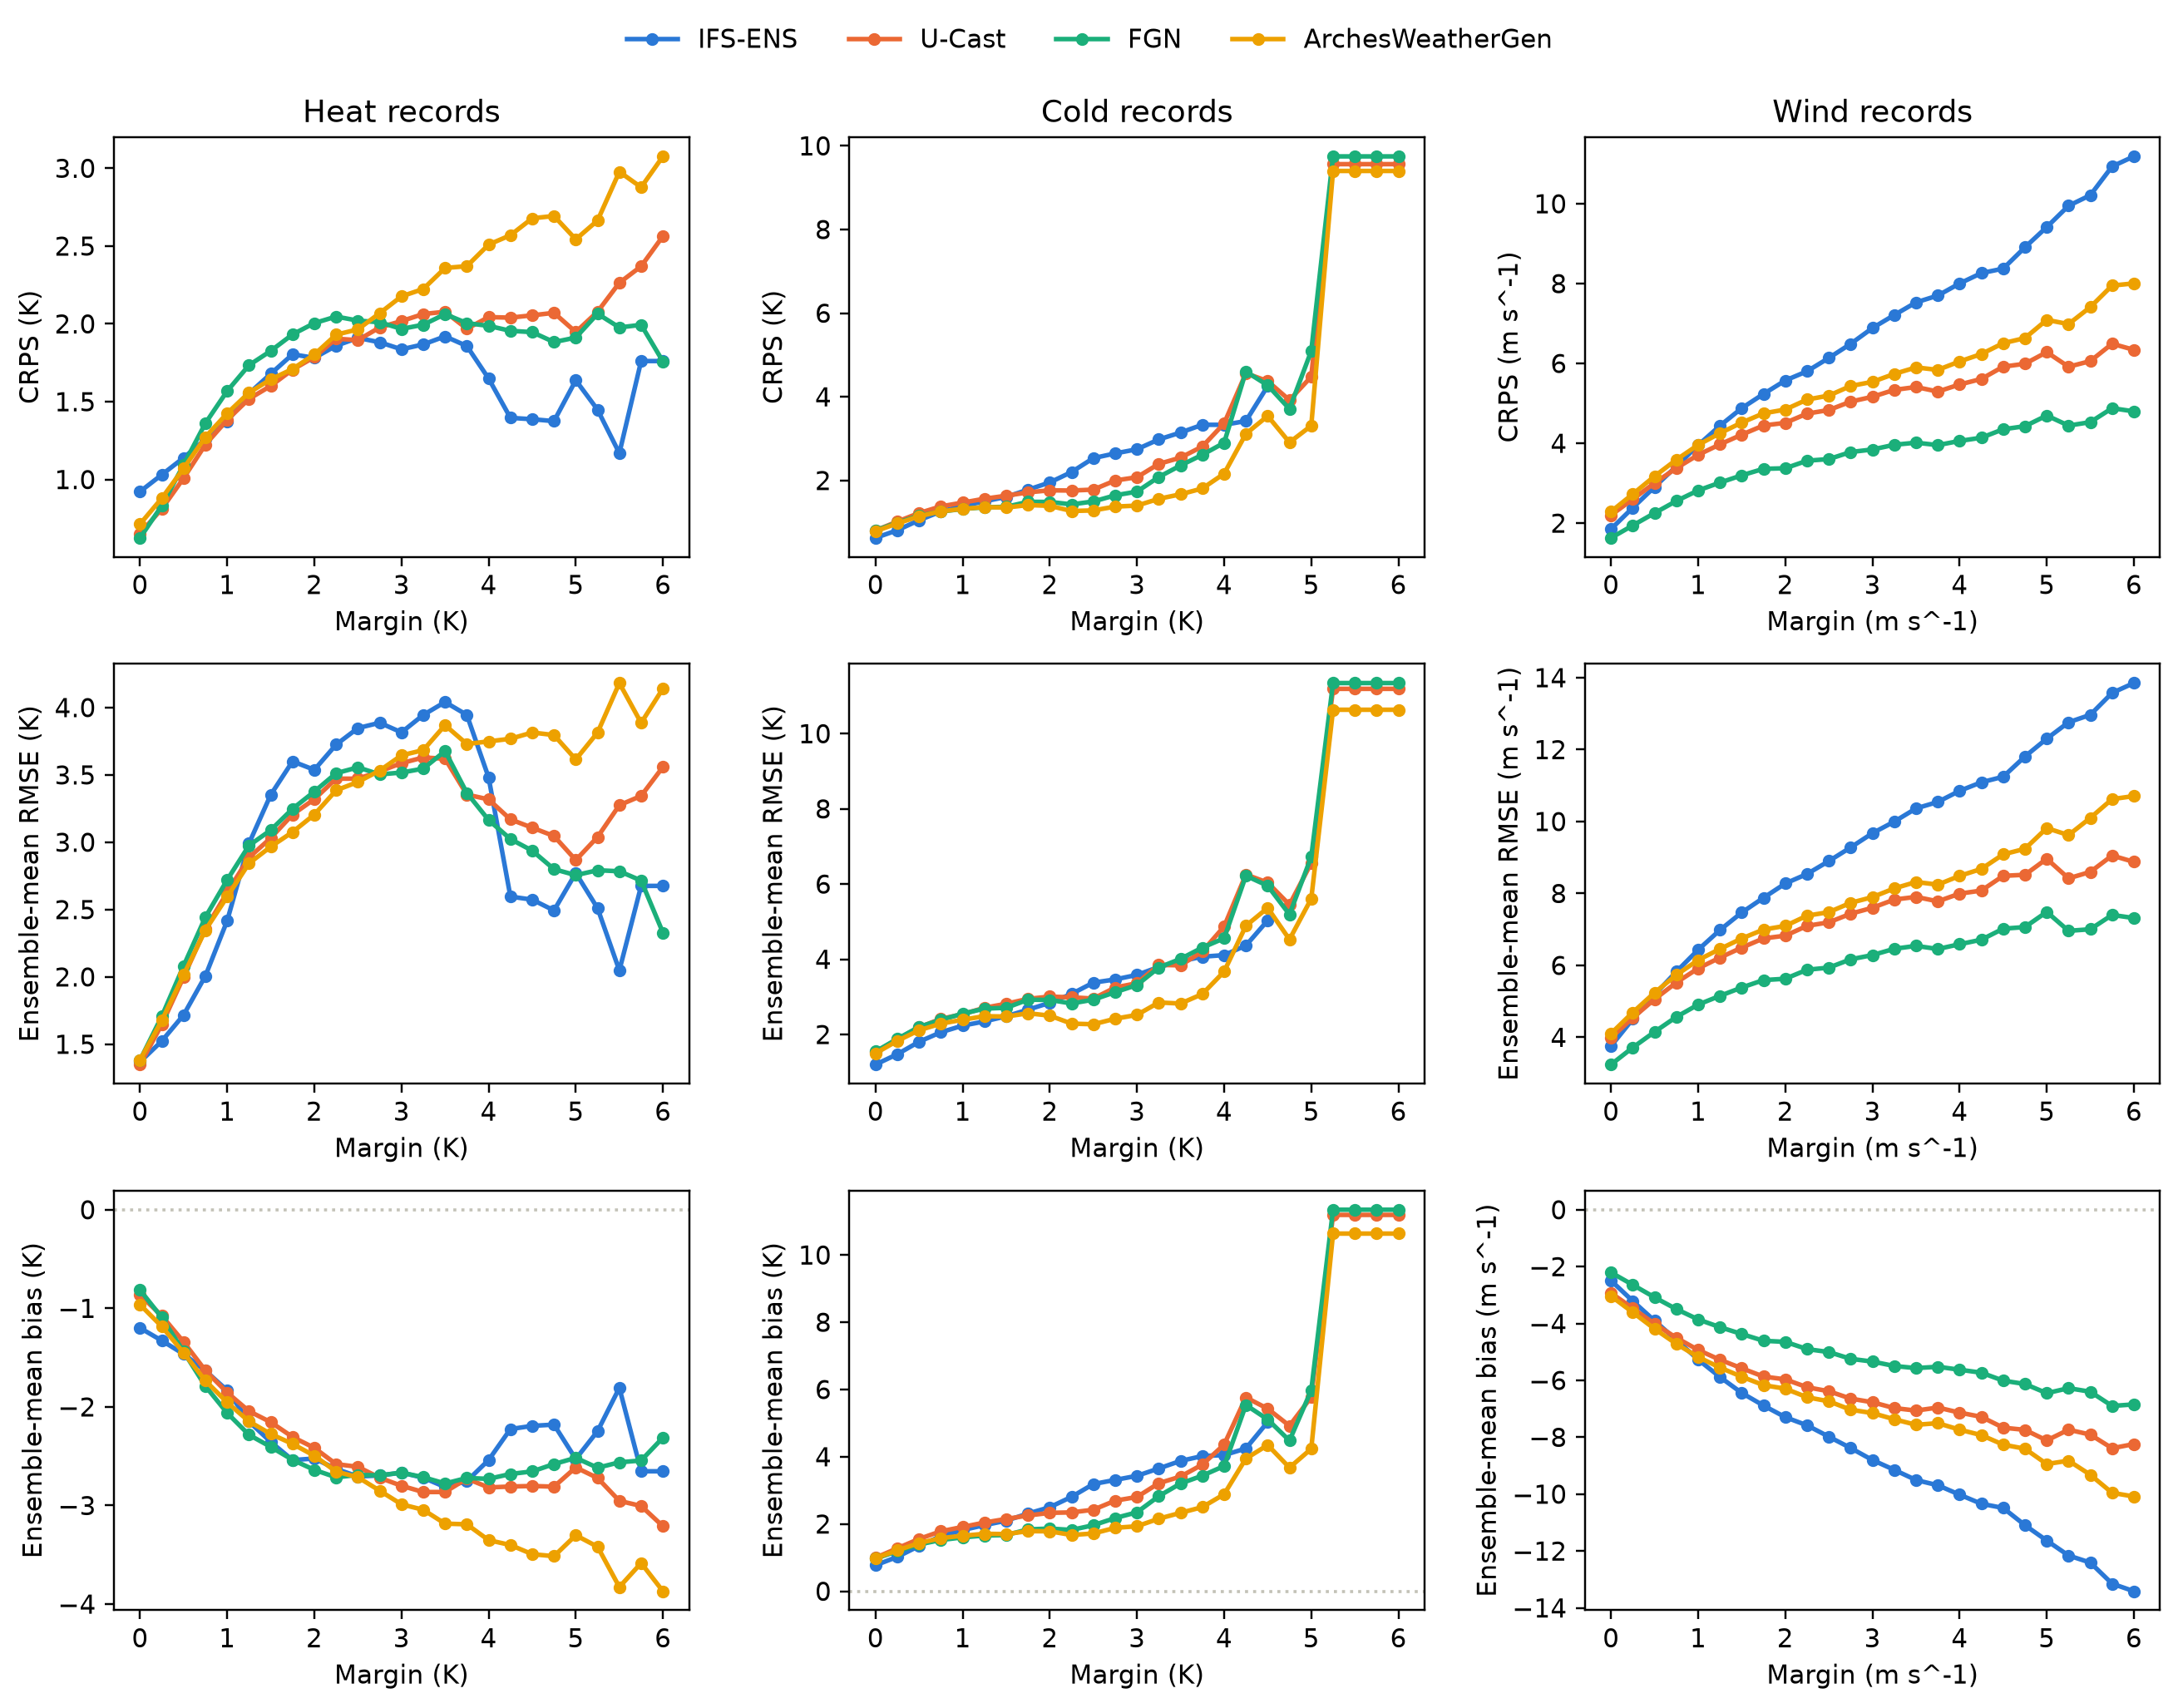
\includegraphics[width=0.96\linewidth]{fig/margin_intensity_120h_all.png}
\caption{All-domain, all-season margin-conditioned intensity diagnostics at 120 h. Rows show CRPS, ensemble-mean RMSE, and ensemble-mean bias for records exceeding each margin threshold.}
\label{fig:margin-intensity}
\end{figure}

\begin{figure}[t]
\centering
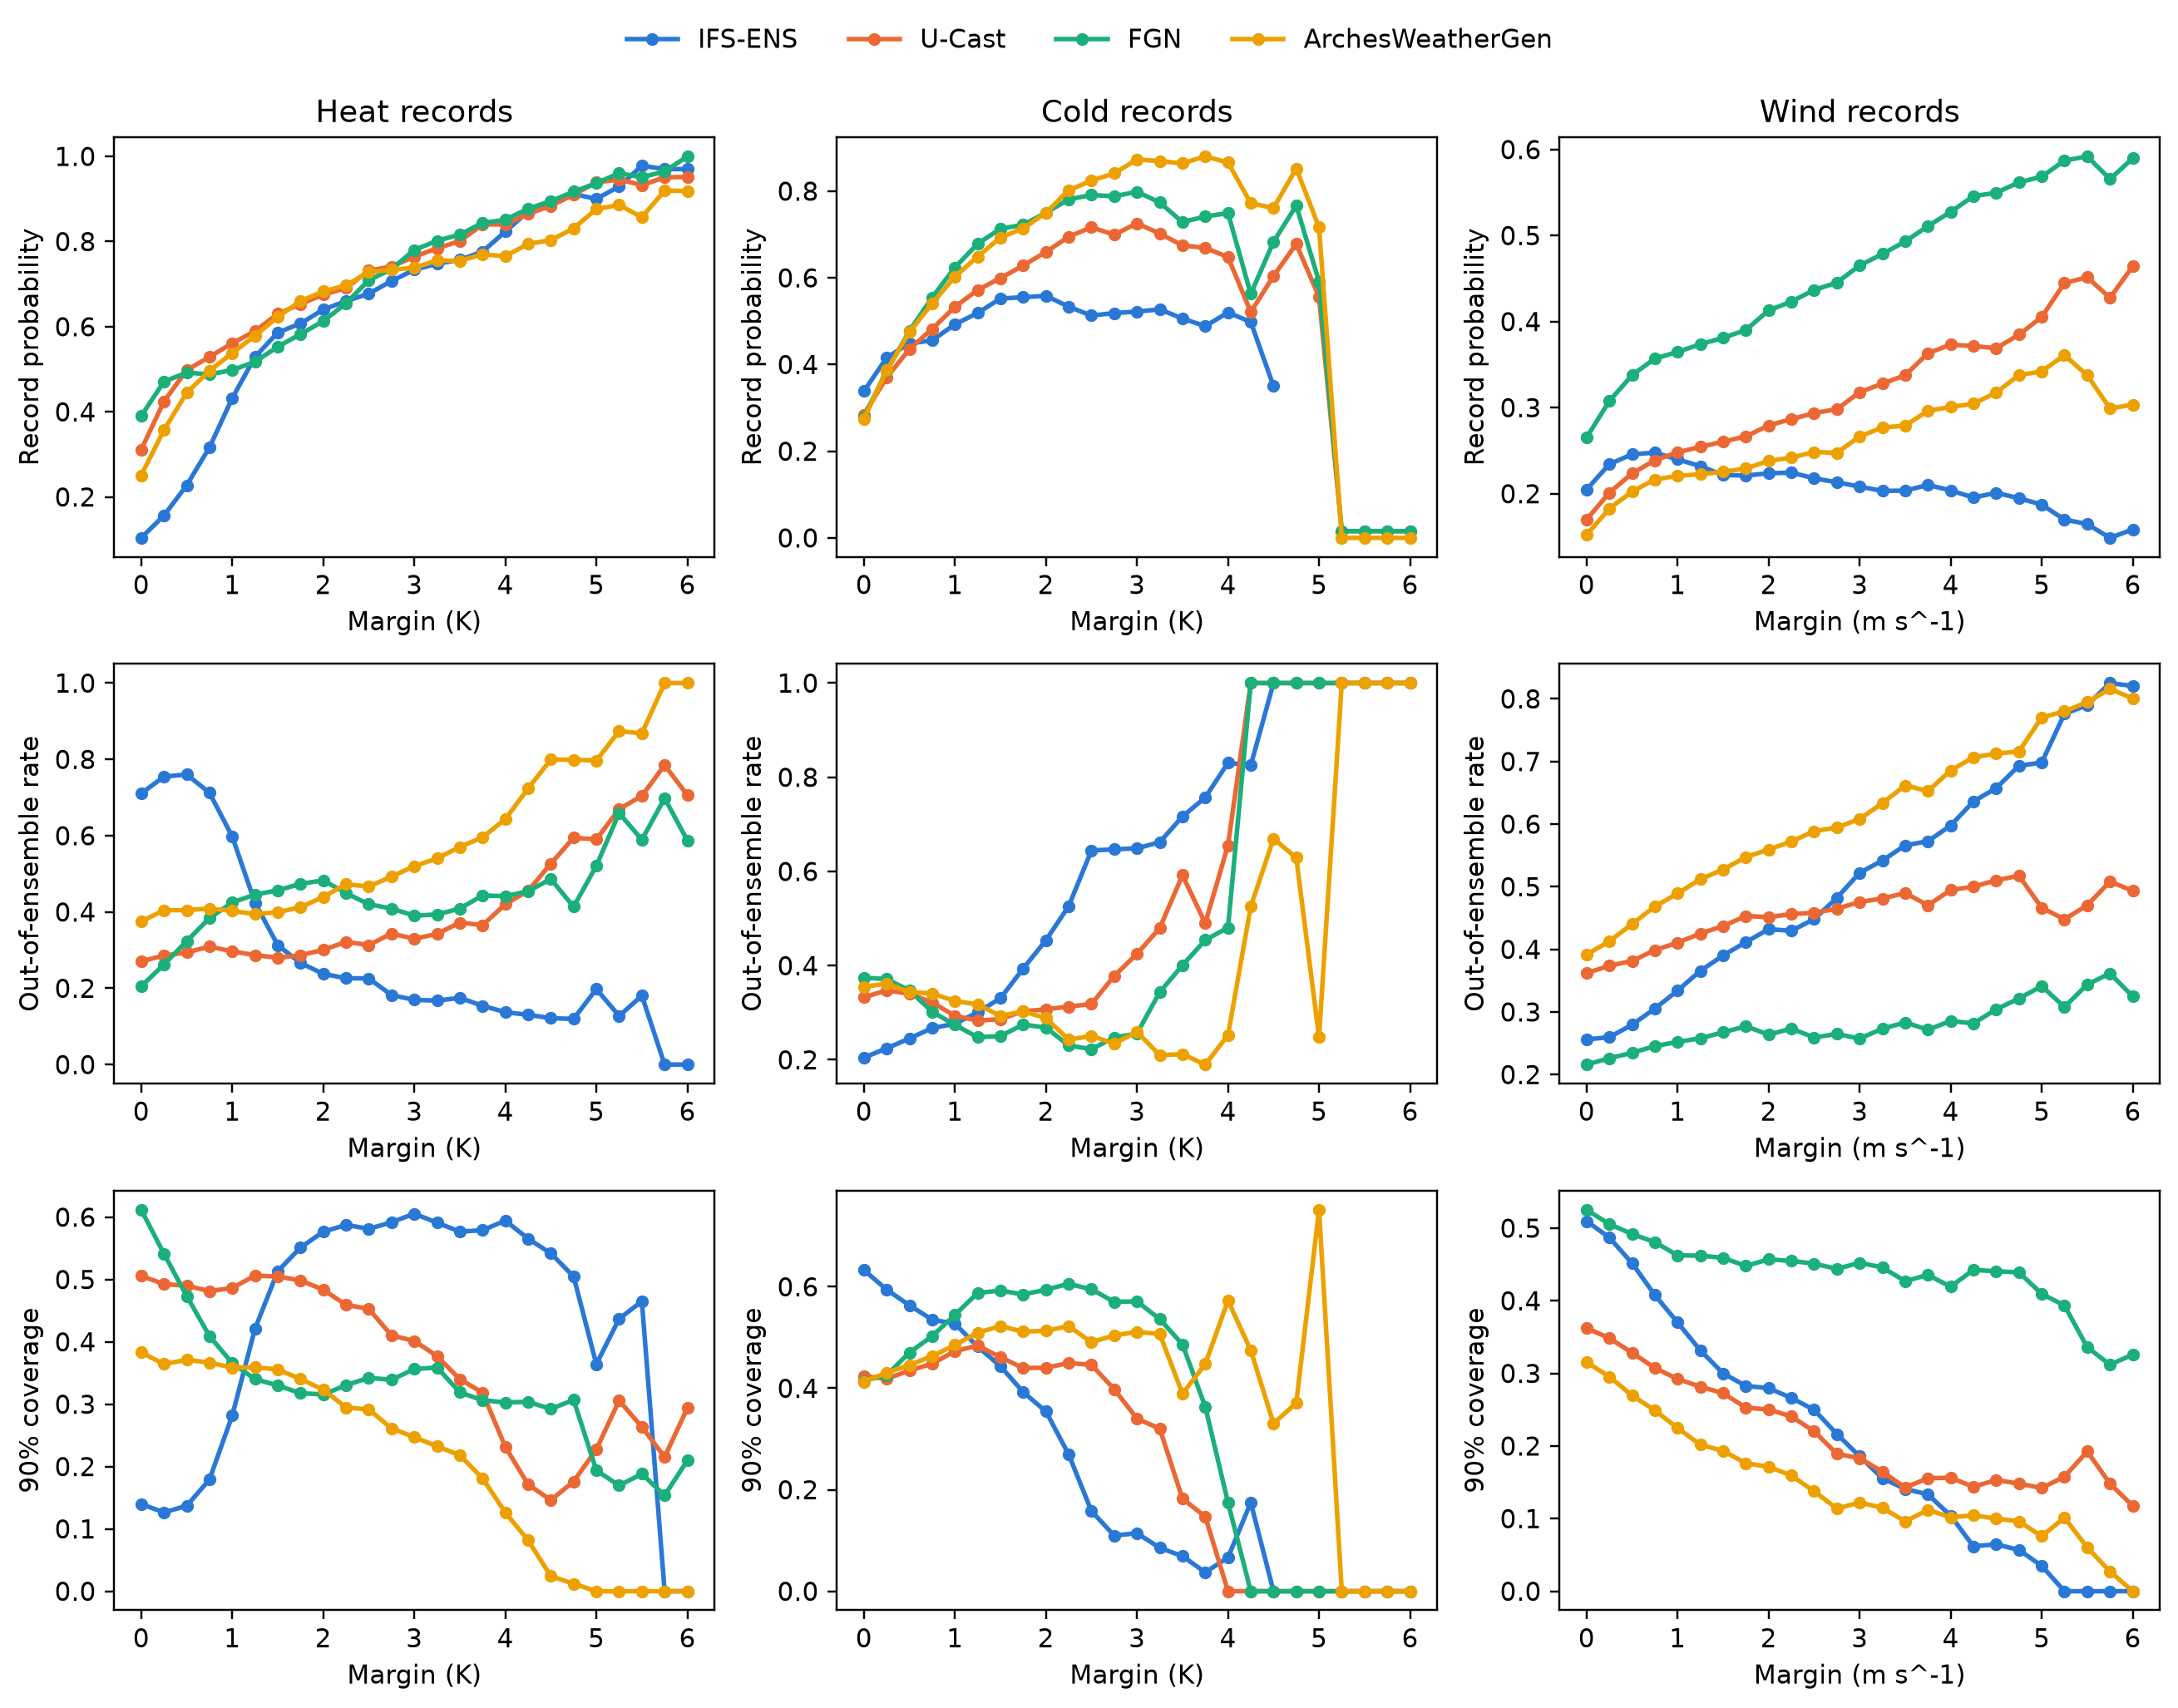
\includegraphics[width=0.96\linewidth]{fig/margin_probabilistic_120h_all.png}
\caption{All-domain, all-season margin-conditioned probabilistic diagnostics at 120 h. Rows show mean record probability, out-of-ensemble rate, and empirical 90\% coverage.}
\label{fig:margin-probabilistic}
\end{figure}

\section{Discussion}

Record-breaking extremes are a stringent benchmark because they combine rarity, societal relevance, and extrapolation beyond local seasonal history. Deterministic AI forecasts can be highly skillful on average while attenuating records \citep{zhang2026recordextremes}. Probabilistic AI forecasts change the question but do not remove the need for direct tail evaluation. An ensemble may improve on deterministic soft-cap behavior by assigning probability mass beyond the historical record, yet still fail by remaining underdispersive, by concentrating support just above the threshold rather than near the observed intensity, or by issuing poorly calibrated high probabilities.

The present diagnostics separate those possibilities. Point-summary RMSE and bias reveal whether the center of the ensemble inherits deterministic attenuation. Expected-minus-observed counts indicate whether records are over- or underforecast in expectation. Brier scores and reliability summaries ask whether record probabilities are numerically usable. Zero-probability miss rates identify cases for which the ensemble never entered the record side of the threshold. CRPS evaluates the full predictive distribution, and margin-conditioned out-of-ensemble and coverage diagnostics ask whether the distribution reaches the observed intensity of the most unprecedented events. Together, these diagnostics show that probabilistic record forecasting should be evaluated on at least two levels: threshold support and intensity support.

Three findings stand out from the current result set. First, record-breaking events are a distinct probabilistic verification regime. Scores that look strong for average weather can degrade sharply when evaluation is restricted to unprecedented events. Second, forecast behavior is strongly structured by event type, lead time, season, and land-sea class. Long-lead JJA land heat records, DJF land cold records, and wind records over sea points do not behave like interchangeable subsets of one common tail problem. Third, margin-conditioned diagnostics show why record probability alone is insufficient. Several models retain substantial mean probability of threshold exceedance while simultaneously losing coverage and exhibiting higher out-of-ensemble rates in the largest-margin subsets.

At the same time, the current manuscript should be read with several methodological cautions in mind. The most immediate is verification. ERA5 is a high-quality global reanalysis and a practical common benchmark, but it is not direct observation, and its uncertainty varies by variable and region \citep{hersbach2020era5, rasp2024weatherbench2}. HRES-fc0 is a sensible operational reference, but mixed verification targets complicate direct model ranking. A second caution is temporal scope. The present analysis emphasizes the 2022 processed outputs, which are already scientifically informative but do not yet establish year-to-year robustness. A third caution is dependence. Record events cluster in space and time because individual heatwaves, cold-air outbreaks, and storm systems generate many neighboring record grid-time points. Confidence intervals based on block or event-level resampling are therefore a priority extension.

Several near-term improvements are already supported by the current workflow. The occurrence figure and table presented here summarize only one common lead and can be expanded in the Supplementary Information to cover every processed lead, season, and land-sea class. The margin files contain all ingredients needed for a dedicated coverage and out-of-ensemble panel across multiple lead times. Median-based point and margin diagnostics are also available and are natural supplement material. Beyond presentation, the most important scientific extensions are multi-year evaluation, common-verification sensitivity analysis, forecast-conditioned diagnostics for the forecaster's dilemma, and uncertainty quantification that respects spatiotemporal dependence.

\section{Conclusions}

We presented a probabilistic benchmark for record-breaking heat, cold, and wind that extends the deterministic record-extreme framework of \citet{zhang2026recordextremes} to ensemble weather forecasts. Using 2022 forecasts from IFS-ENS, FGN, U-Cast, and ArchesWeatherGen, we evaluated point summaries, occurrence probabilities, Brier scores, reliability-related summaries, CRPS, and margin-conditioned tail diagnostics.

The results show that record-breaking extremes are not merely rare versions of average-weather verification. They expose structured weaknesses that depend on event type, lead time, season, and surface regime. Some AI ensembles represent heat-record occurrence and intensity competitively in parts of this design space, but cold records and especially wind records remain substantially more fragile. Most importantly, probabilistic forecast quality cannot be summarized by threshold crossing alone. A useful record forecast must both assign support beyond the historical record and retain enough tail coverage to contain the realized event intensity.

These findings support record-breaking extremes as a standard stress test for probabilistic AI weather forecasts. They also show that progress should be evaluated not only with average skill scores, but with diagnostics that directly test tail calibration, tail support, and tail coverage.

\section*{Data and Code Availability}

The evaluation code is organized under \texttt{download/}, \texttt{eval/}, \texttt{viz/}, and \texttt{job\_scripts/}. Processed score files are stored under \texttt{results/<model>/<metric>/}. A batch plotting script in \texttt{viz/} generates the complete stratified figure inventory under \texttt{manuscript/fig/stratified/}; the occurrence-probability files contain both reliability diagrams and precision-recall curves at the common 48 h lead. Persistent archive links and final data-access instructions will be added before submission.

\section*{Acknowledgments}

\bibliographystyle{plainnat}
\bibliography{main}

\appendix

\section{Supplementary materials}

\end{document}
